% *********************************************************************
% © 2021-2023 Jeremy Sylvestre
%
% Permission is granted to copy, distribute and/or modify this document
% under the terms of the GNU Free Documentation License, Version 1.3 or
% any later version published by the Free Software Foundation; with no
% Invariant Sections, no Front-Cover Texts, and no Back-Cover Texts. A
% copy of the license is included in the appendix entitled “GNU Free
% Documentation License” that appears in the output document of this
% PreTeXt source code. All trademarks™ are the registered® marks of
% their respective owners.
%
% *********************************************************************

\newcommand*{\xmin}{-1.5}
\newcommand*{\xmax}{6.5}
\newcommand*{\ymin}{-0.5}
\newcommand*{\ymax}{5.5}

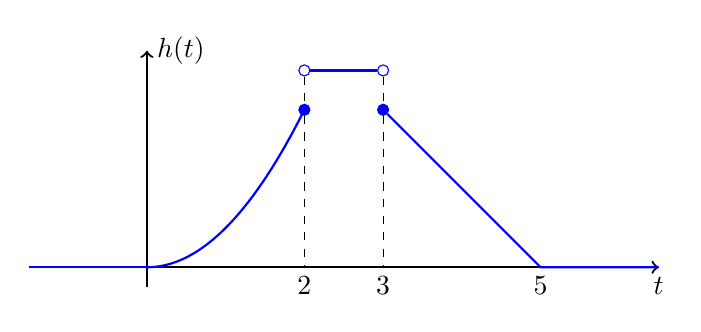
\begin{tikzpicture}
[
	closedpt/.style={circle,draw,fill,inner sep=0pt,minimum size=4pt},
	openpt/.style={circle,draw,inner sep=0pt,minimum size=4pt},
	yscale=0.5
]

	% axes
	\draw[->,thick] (\xmin,0) -- (\xmax,0) node[below] {$t$};
	\draw[->,thick] (0,\ymin) -- (0,\ymax) node[right] {$h(t)$};

	% graph
	\draw[thick,blue] (\xmin,0) -- (0,0);
	\draw[thick, blue, domain=0:2, smooth] plot (\x,{\x * \x});
	\node[closedpt,blue] at (2,4) (p) {};

	\node[openpt,blue] at (2,5) (c1) {};
	\node[openpt,blue] at (3,5) (c2) {};
	\draw[thick, blue] (c1) -- (c2);

	\node[closedpt,blue] at (3,4) (l) {};

	\draw[thick,blue] (l) -- (5,0) -- (\xmax,0);

	\draw[dashed] (c1) -- (p) -- (2,0) node[below] {$2$};
	\draw[dashed] (c2) -- (l) -- (3,0) node[below] {$3$};
	\node[below] at (5,0) {$5$};

\end{tikzpicture}
